\subsection{Aufbau}
In Abbildung \ref{fig:Aufbau} ist der Aufbau eines Geiger-Müller-Zählrohrs zu sehen. Es besteht aus einer Anode und einer Kathode, die zusammen einen Zylinderkondensator bilden. Das Elektrische Feld ist radialsymmetrisch
\begin{align}
	E(r) = \frac{U}{r\ln(\frac{r_\text{k}}{r_\text{a}})} \ .
\end{align}
In Abbildung \ref{fig:Aufbau} fallen die Teilchen durch das Eintrittsfenster von links in das Zählrohrvolumen ein. Es ist mit Edelgas gefüllt, das durch die Strahlung ionisiert werden soll. Da Strahlung stark mit Materie wechselwirkt sollte das Eintrittsfenster, wie in der Abbildung eingezeichnet, aus einem \glqq dünnwandigen Material mit Atomen niedriger Ordnungszahl\grqq\cite[Kap. 5]{\V} (Mylar-Folie) bestehen. Alternativ könnte die Kathode auch aus einer Drahtspirale bestehen durch dessen Windungen sich die Teilchen bewegen können.
\begin{figure}[h!]
	\centering
	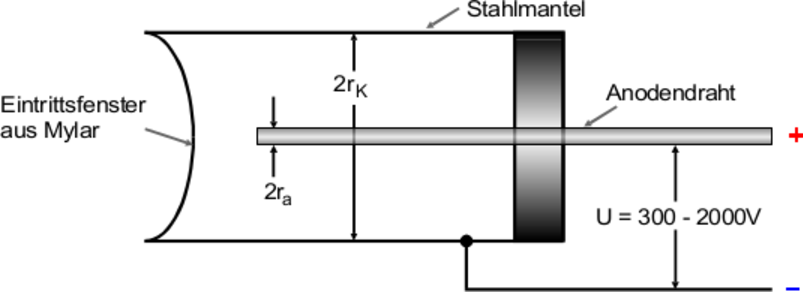
\includegraphics[width=0.45\textwidth]{Aufbau.pdf}
	\caption{Grundsätzlicher Aufbau eines Geiger-Müller-Zählrohrs \cite{\V}}
	\label{fig:Aufbau}
\end{figure}
\subsection{Funktionsweise}
\todo[color=red,inline]{Das Teilchen ist doch geladen, wird also durch das elektrische Feld zum Draht oder zum Zylinder gezogen. Was ist, wenn das Teilchen an einem der beiden ankommt und noch Energie übrig hat? Bzw. es wird durch das Feld ja sogar beschleunigt. Stößt es sich an der Anode/Kathode ab und bewegt sich weiter? Geht die Energie verloren? Kann das Teilchen dann, wenn es sich nicht mehr fortbewegt auch noch ionisieren? \\ Je nach dem wäre die Energie nicht mehr proportional zur Anzahl.}
Ein geladenes Teilchen, das in das Zählrohr eindringt, ionisiert die Gasatome. Dabei verliert es jedes Mal einen (sehr kleinen) Teil seiner Energie und bewegt sich solange weiter fort, bis seine gesamte Energie aufgebraucht ist. Bei jeder Ionisation entstehen ein Elektron und ein positiv geladener Atomrumpf. Die Anzahl dieser Ionenpaare ist proportional zur ursprünglichen Teilchenenergie.
\subsubsection*{Die Elektronen}
Was nach der Ionisation mit den Elektronen geschieht, hängt von der angelegten Spannung ab. Es können die nachfolgenden Bereiche, die in Abbildung \ref{fig:DependenceVoltage} dargestellt sind, unterschieden werden.
\begin{itemize}
	\item[\textbf{I}] Ist die Spannung klein, reicht die Beschleunigung des elektrischen Felds nicht aus, um die Elektronen bis zur Anode zu bringen. Die meisten rekombinieren vorher mit den Atomrümpfen. Mit ansteigender Spannung sinkt die Rekombinationswahrscheinlichkeit schnell ab.
	\item[\textbf{II}] Irgendwann ist die Spannung so groß, dass quasi alle Elektronen den Draht erreichen. Dann ist der zwischen Anode und Kathode fließende Strom proportional zu Energie und Intensität der Strahlung. In diesem Bereich kann man das Rohr auch als Ionisationskammer bezeichnen.
	\item[\textbf{III}] Die Elektronen werden auf dem Weg zum Draht immer stärker beschleunigt. Es gibt einen Spannungswert, ab dem ihre Energie groß genug ist, um ihrerseits wieder Atome durch Stöße zu ionisieren (Stoßionisation). Die Zahl der Ionisationen steigt lawinenartig an, man spricht hierbei von einer Townsend-Lawine. Die Ladungsmenge $Q = n\cdot e$, die pro einfallendem Strahlungsteilchen am Draht ankommt, ist nun ausreichend groß, um einen messbaren Stromimpuls zu verursachen. Da $Q$ und somit auch der Strompuls nach wie vor proportional zur Energie (und Intensität) der Strahlung ist, spricht man von einem Proportionalzählrohr.
	\item[\textbf{IV}] Die Spannung ist schließlich so groß, dass die Energie der Elektronen ausreicht, um durch inelastisches Stoßen die Atome anzuregen, die deshalb UV-Photonen emittieren. Die Photonen haben genug Energie, um Atome zu ionisieren. Da sie allerdings elektrisch neutral sind können sie sich auch senkrecht zum elektrischen Feld bewegen. Die Ionisationslawinen finden nun nicht mehr nur lokal, sondern im gesamten Volumen des Zylinders statt. Die am Draht ankommende Ladung $Q$ ist jetzt nur noch proportional zur Intensität, nicht mehr zur Energie der Strahlung. Da der durch $Q$ verursachte Strom so groß ist, dass er leicht detektiert werden kann, ist dieser Bereich gut für die Intensitätsmessung von Strahlung geeignet. Hier ist auch der eigentliche Arbeitsbereich des Geiger-Müller-Zählrohrs.
\end{itemize}
\begin{figure}[h!]
	\centering
	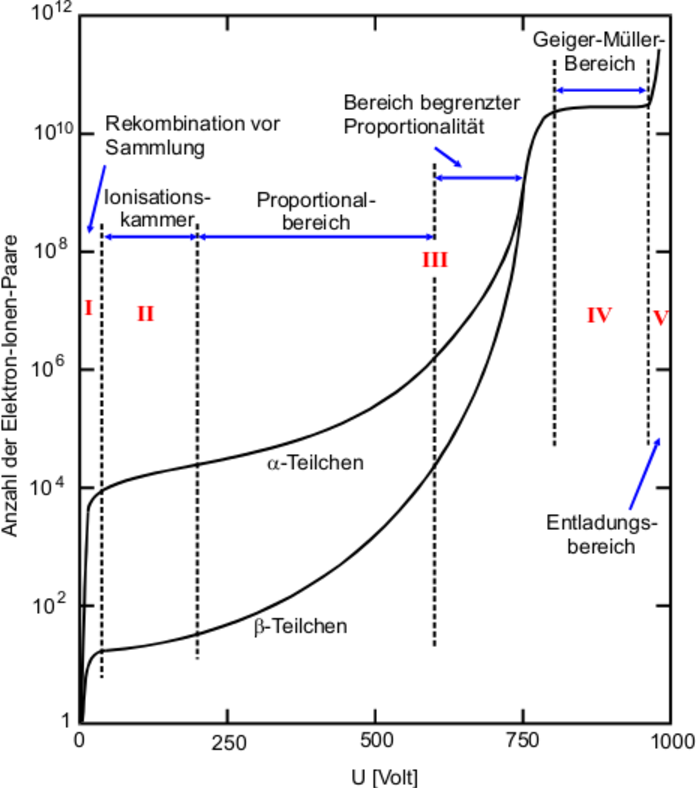
\includegraphics[width=0.5\textwidth]{Spannungsabhangigkeit.pdf}
	\caption{Anzahl der durch Ionisation frei gewordene Elektronen in Abhängigkeit von der angelegten Spannung}
	\label{fig:DependenceVoltage}
\end{figure}
\subsubsection*{Die Atomrümpfe}
Die Ionen können aufgrund ihrer großen Masse nicht so schnell zur Kathode wandern, wie die Elektronen zum Draht. Durch ihre positive Ladung schwächen sie das elektrische Feld ab, sodass es für eine Zeit $T$ nicht mehr zu Stoßionisationen kommen kann. Das heißt es kann keine Elektronenlawine und keine Photonen-Emissionen geben und ein einfallendes Teilchen kann nicht detektiert werden. Deshalb wird $T$ auch Totzeit genannt. \\
Die Ionen bewegen sich zur Kathode und die effektive Feldstärke steigt an. Es beginnt die Erholungszeit $T_\text{E}$, in der wieder Elektronenlawinen möglich sind. Allerdings werden die Ionen an der Zylinderwand nicht nur neutralisiert, sondern lösen auch durch Stoß Elektronen aus der Metalloberläche aus. Diese Sekundärelektronen werden beschleunigt und ionisieren Atome, sodass erneut mehrere Ipulse detektiert werden, die aber nicht von Strahlung verursacht wurden. Dieser Vorgang wird als Nachentladung bezeichnet. \\
Durch Zugabe von Alkoholdampf in das Zählrohr können die Nachentladungen gemindert werden. Dann stoßen die ionisierten Atomrümpfe auf ihrem Weg zur Kathode mit den Alkoholmolekülen und da die Ionisierungsenergie des Alkohols kleiner ist, als die der Ionen, werden die Alkoholmoleküle ionisiert. Sie wandern statt den Atomrümpfen zur Kathode und werden dort neutralisiert. Ihre Energie reicht nicht aus um noch ein Elektron aus der Kathode zu schlagen, sondern geht in die Molekülschwingung. Ist die angelegte Spannung allerdings zu hoch, kommt es auch bei den Alkoholmolekülen zu zahlreichen Nachentladungen, die in eine Dauerentladung über gehen und durch den ständig fließenden hohen Strom das Zählrohr zerstören (Bereich \textbf{V} in Abb. \ref{fig:DependenceVoltage}).
\subsubsection*{Charakteristik}
Als Charakteristik eines Zählrohrs bezeichnet man die Abhängigkeit der registrierten Elektronen am Draht in Abhängigkeit von der angelegten Spannung, bei konstanter Strahlungsintensität. Das in Abbildung \ref{fig:Charakteristik} eingezeichnete Plateau ist ein Maß für die Güte des Zählrohrs. Je flacher und länger, desto besser, jedoch ist eine Steigung von Null ein Ideal, das aufgrund von Nachentladungen selbst mit Alkoholdampf nicht erreichbar ist.
\begin{figure}[h!]
	\centering
	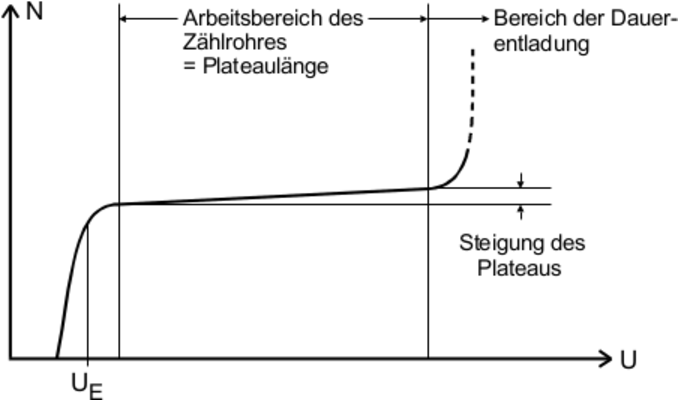
\includegraphics[width=0.6\textwidth]{Charakteristik.pdf}
	\caption{Charakteristik eines Zählrohrs}
	\label{fig:Charakteristik}
\end{figure}